\section{Challenges}
\label{chal}
There are several challenges to be addressed when designing a benchmarking framework for SDPSs. In this section, we analyze these challenges and explain our solutions.

\begin{figure*}
    \centering
    \begin{subfigure}[b]{0.32\textwidth}
        \includegraphics[width=\textwidth]{eps/no_queue}
        \caption{Without message queue}
        \label{fig_no_queue}
    \end{subfigure}
    ~ %add desired spacing between images, e. g. ~, \quad, \qquad, \hfill etc. 
      %(or a blank line to force the subfigure onto a new line)
    \begin{subfigure}[b]{0.32\textwidth}
        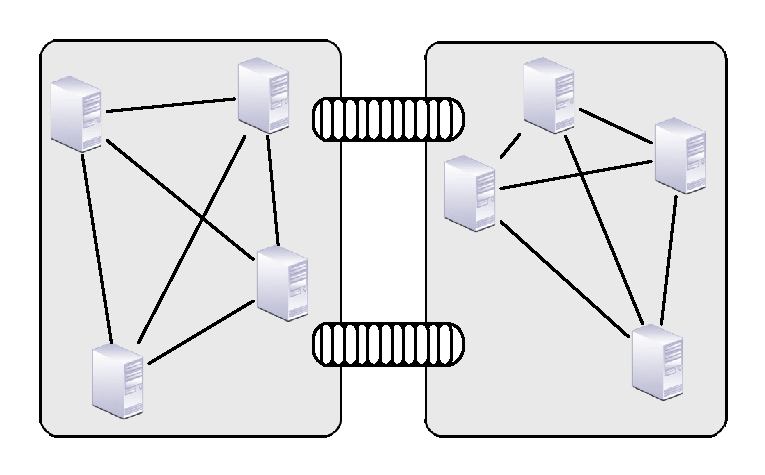
\includegraphics[width=\textwidth]{eps/yes_queue}
        \caption{With message queue}
        \label{fig_yes_queue}
    \end{subfigure}
    \begin{subfigure}[b]{0.32\textwidth}
        \includegraphics[width=\textwidth]{eps/node_queue}
        \caption{Partial message queue}
        \label{fig_partial_queue}
    \end{subfigure}
        \caption{Different system designs to connect data generator and SUT. \todo[inline]{O really do not get what the thunders represent and what this figure wants to present.}}
            \label{fig_queue_link}
\end{figure*}



\para{ \textit{Simplicity is key}}. The first challenge is to design a simple benchmarking framework as complex benchmarking frameworks can  cause  additional overheads. \todo[inline]{The number of components is not the only factor determining system complexity. Generally, I would prfer an argument on efficiency or low overhead than simplicity.=> deleted ambiguous part of sentence} \todo[inline]{AK: I really do not buy this argument of simplicity. Plus, "can cause additional overheads" without concrete reasons why, is very weak here.}

For example, the connection between the data generator and the SUT can cause large additional overheads when benchmarking.  To test the stream data processing engine, a data generator component is essential, to provide large amounts of streaming data. Figure \ref{fig_queue_link} shows  three possible cases to link the data generator and the SUT. The simplest design is to connect the SDPS directly to the data generators as shown in Figure \ref{fig_no_queue}. Although this is a perfectly acceptable design, it does not match real-life use-cases. In large-scale setups, stream data processing engines do not connect to push-based data sources but pull data from distributed message queues. A pull based design, where data sources and SUT are connected through queues, is in Figure \ref{fig_yes_queue}. A common bottleneck of this option is the throughput of the message queuing system. Also, this adds  a de-/serialization layer between the SUT and the data sources. Therefore, we use a third option, which is a hybrid of the first two. As can be seen in Figure \ref{fig_partial_queue}, we embed the queues as a separate module in the data generators. This way, the throughput is bounded only by the network bandwidth and the systems work more efficiently as there are no de-/serialization overheads.%\todo[inline]{not as simple as no queue...=>deleted sentence}


\para{ \textit{Separate driver and tested system}}. The second challenge is to isolate the  driver from the SUT as much as possible. In previous works, researchers measured the throughput  either  inside the SUT, or used internal statistics of the SUT. % or just do not mention about the measurement details. 
However, if the measurements and SUT are not separated, then the measurement computations can influence the results of benchmark.
In our benchmarking framework, we separate the driver and SUT for each measurement metric and perform measurements separately from the SUT. 
%\todo[inline]{I don't know what you want to say in this sentence. why would you associate the KPI/metric with a unit under test and what does that mean?-> I explained it in following sentences.}


The first metric is throughput. 
If the system can ingest and process all the data produced by the driver instances during the whole experiment, then the system can \textit{sustain} the given throughput and we call it \textit{sustainable throughput}. If the system sustains the given throughput and cannot process more, then we call it \textit{maximum sustainable throughput}. In this paper, we analyze the maximum sustainable throughput of SDPSs which is  sum of the throughputs of all driver instances. So, we keep throughput assessment inside driver instances and sum them at the end of experiment. 

\todo[inline]{AK: Please explain the throughot concept better or refer to where in the paper this is explained.}

  
The second evaluation is latency. We define the latency of a tuple to be the interval between tuple's event time and emission time from SUT's sink operator. We develop a model to calculate the latency of stateful operator  which we analyze in Section \ref{sec_latency}.
%\todo[inline]{I like the concept of isolating the driver, however, separating would be a better term. But the description of this separation is completely unclear. Also, if it is required to separate, you should explain why and how we did it. You have some of the why but none of the how=>fixed}

\para{ \textit{Unreal latency and throughout}}.
The third challenge is to measure the metrics with close to real-life scenarios. %\todo[inline]{This is repetitive, you need to mention real world only once in this paragraph=>fixed} 
One example  is the throughput measurement. In the previous SDPS benchmarks, the throughput of a SUT is measured by either taking quantiles over the test duration, or showing max, min, and average results. 
%\todo[inline]{Why? And what do you mean by reason about the SUT. This sentence needs to be rewritten => deleted sentence}
From a user's perspective on the other hand, the system's throughput is the upper limit throughput that it can sustain in a realistic setup. 
We propose user-defined sustainability policies in our benchmarking framework. For example, the benchmarking framework can take into account the backpressure of  the SUT.  %\todo[inline]{Again repetitive and convoluted, make the text simple and say right away what you want to say instead of incrementally adding parts=>fixed}

\todo[inline]{AK: I really don't get what unreal throughput is and why we use this term. I did not see it anywhere else so far.}


Another example for this challenge is latency measurement. If there are additional systems between the SDPS and data source (driver), then those are likely to add an extra latency for each tuple.  One solution is  to measure the latency in the SDPS the same way as it is measured in batch data processing systems. In this case, the number and complexity of the systems between SDPS and data source is irrelevant as the latency is the interval between tuples' ingestion and output from SUT. However, this measurement of latency is too \textit{optimistic} and does not result in the real latency of the tuple. The reason is that  the actual latency is based on tuples' event generation time. For example in online games, the event time can be a user's specific action in a game, the latency then is the time interval between user's action and the result being emitted from the SDPS. Therefore, the usual method of measuring the latency within SDPS does not conform to real world scenarios especially in pull-based SDPSs. Depending on their backpressure mechanism, a pull-based SDPS will reduce the input rate on high loads, which will not be reflected in the measured latency. To solve this, we define the latency for SDPSs to be the difference between tuple's event time and output time. 

Another factor triggering the unrealistic latency is the data generation rate. If the input data rate is higher than the SDPS's \textit{maximum sustainable throughput} and we measure the event time latency, the results may not exhibit the real  latency. 
Initially the system will try to ingest as much data as possible. As a result, the SUT's processing time will take longer and the latency will increase for every adjacent tuple. To solve this issue, we conduct experiments with the maximum sustainable throughput for each SDPS. 
%\todo[inline]{The previous text is confusing. Try to make it simple and precise}
%\todo[inline]{What does associate mean?->deleted}
%\todo[inline]{Repetition=>fixed}
%\todo[inline]{This means we do not measure system latency? Then this is a component benchmark and cannot report on application level performance. This is also contradictory to previous discussions about the separation of driver and sut=>rewritten above}
%\todo[inline]{I think this was written several times already.=>rewritten above}   \todo[inline]{Again, repetition. Please concentrate on the message this section is supposed to convey. This would be the challenge of measuring latency. I have not clearly read your solution to the problem.=>rewritten above}


\para{ \textit{Latency of stateful operators}} The final challenge is measuring the latency of stateful operators. Up to this point, the related work either concentrated on stateless operators or evaluated the latency of stateful operators by checkpointing to external systems. As we discussed above, this approach can be a bottleneck and will influence the measurements. In our benchmarking framework, we propose a solution to this problem.  
We aggregate tuples by selecting their maximum timestamp and append the resulting timestamp to the emitted tuple from stateful operator. 
 In this way, we measure the latency of stateful computation time, excluding the tuples' waiting time (in window) in stateful operator. 

%\todo[inline]{Did we remove the formal definition, then this should be updated=>fixed}

